\documentclass[12pt]{article}
\usepackage[english]{babel}
\usepackage{natbib}
\usepackage{url}
\usepackage[utf8x]{inputenc}
\usepackage{amsmath}
\usepackage{graphicx}
\graphicspath{{images/}}
\usepackage{parskip}
\usepackage{fancyhdr}
\usepackage{vmargin}
\usepackage{xcolor}
\usepackage{siunitx}
\usepackage{physics}
\setmarginsrb{3 cm}{2 cm}{3 cm}{2 cm}{1 cm}{1.5 cm}{1 cm}{1.5 cm}

\title{Lab 09}													% Title
\author{G 03}														% Author
\date{04 june 2019}														% Date

\makeatletter
\let\thetitle\@title
\let\theauthor\@author
\let\thedate\@date
\makeatother

\pagestyle{fancy}
\fancyhf{}
\rhead{\theauthor}
\lhead{\thetitle}
\cfoot{\thepage}
\newcommand{\mis}[3]{(#1 \pm #2) \ #3}
\newcommand{\misp}[3]{(#1 \#3 \pm #2}
\begin{document}

%%%%%%%%%%%%%%%%%%%%%%%%%%%%%%%%%%%%%%%%%%%%%%%%%%%%%%%%%%%%%%%%%%%%%%%%%%%%%%%%%%%%%%%%%

\begin{titlepage}
	\centering
    \vspace*{0.5 cm}
    
\includegraphics[scale = 0.75]{polito.jpg}\\[1.0 cm]				% University Logo
    \textsc{\LARGE Politecnico di Torino}\\[2.0 cm]						% University Name
	\textsc{\Large Digital systems electronics\\ A.A. 2018/2019}\\[0.5 cm]		% Course Code
	\textsc{\Large Prof. G. Masera}\\[0.5 cm]		% Nome del Professore
	\rule{\linewidth}{0.2 mm} \\[0.4 cm]
	{ \huge \bfseries \thetitle \\ \small \thedate}\\
	\rule{\linewidth}{0.2 mm} \\[1.5 cm]
	
	\begin{minipage}{0.4\textwidth}
		\begin{flushleft} \large
			Berchialla Luca\\												%Cognomi e nomi
			Laurasi Gjergji
			\\
			
			Mattei Andrea\\
            Lombardo Domenico Maria\\
            Wylezek Karolina
            
			\end{flushleft}
			\end{minipage}~
			\begin{minipage}{0.4\textwidth}
            
			\begin{flushright} \large
			236032\\													%Matricole
			238259\\
            233755\\
            233959\\
            267219\\
            
		\end{flushright}
        
	\end{minipage}\\[2 cm]
	
\end{titlepage}

%%%%%%%%%%%%%%%%%%%%%%%%%%%%%%%%%%%%%%%%%%%%%%%%%%%%%%%%%%%%%%%%%%%%%%%%%%%%%%%%%%%%%%%%%
\newpage
\section*{Output compare VS Reload}
{
	
	In the following report the Output Compare register and/or auto-reload register can be calculated from the desired asserted flag frequency using the following formula:
	\[F_{X}=\frac{F_{CLK}}{(OC+1)\cdot(ARR+1)}\;\;\;\;\; (1)\] 
	
	Notice that to correctly generate a square wave with a desired frequency $F_{X}$ exploiting the OC or ARR approach, the formula 1 should also be divided by a 2 factor.
}

\section*{1 - Interrupt-based variable frequency square waveform generator}

In the following section a variable frequency square wave has been implemented exploiting the interrupt approach. 
\[ delta1 = (OCmax1 - OCmin1) * lettura/ADCmax + OCmin1;\]
 
\begin{figure}[h!]
	\centering
	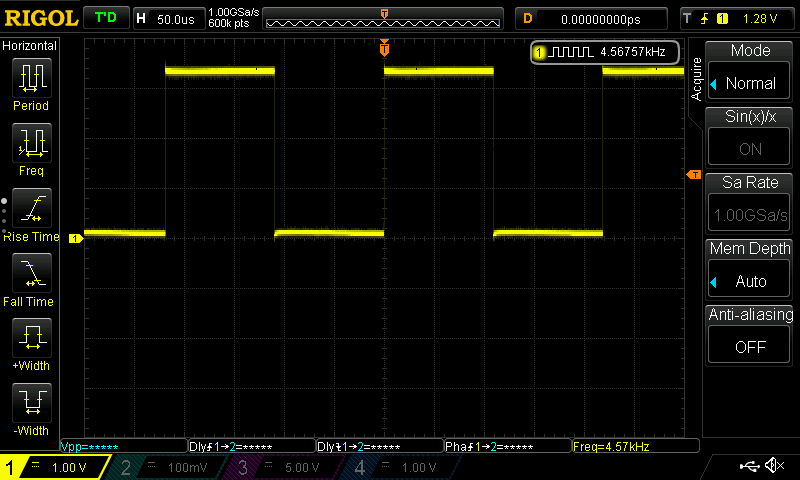
\includegraphics[scale = 0.4]{immagini/DS1Z_QuickPrint10.png}
	\caption{}
\end{figure}
\begin{figure}[h!]
	\centering
	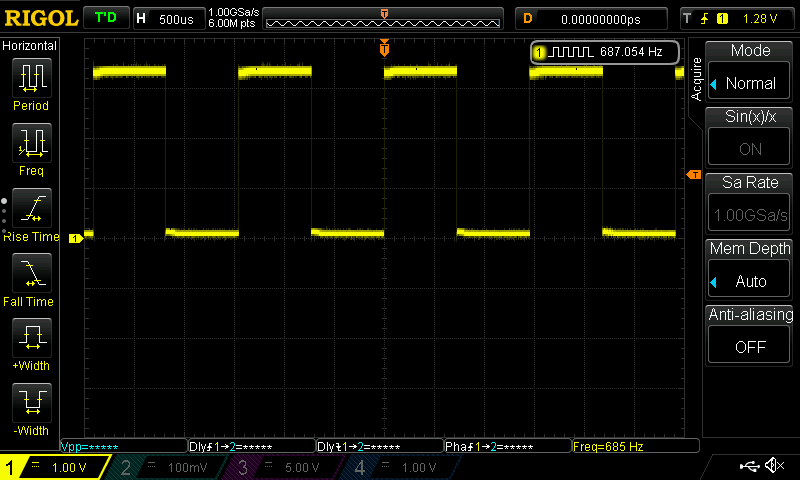
\includegraphics[scale = 0.4]{immagini/DS1Z_QuickPrint11.png}
	\caption{}
\end{figure}


sono molto più stabili
no jitter sensa systick, piccolo jitter con systik


\section*{2.1}

image 12 -13 -11

\section*{2.2 }
il jitter non è apprezzabile perche l'isr è corta???

\section*{2.3 }
image 14 min
image 15 max

\end{document}




